\documentclass[10pt,onecolumn]{book}

\usepackage{times} % font
\usepackage{graphicx} % picture reference
\usepackage{amsmath} % split of mathematical formulas
\usepackage{amssymb} % special mathematical symbols
\usepackage{geometry} % margin
\usepackage{setspace} % letter-spacing
\usepackage{indentfirst} % indent
\geometry{left=2cm,right=2cm, top=2cm, bottom=2cm}
\usepackage{hyperref} % hyperlink
\usepackage{cite}
\usepackage[sectionbib]{chapterbib}

\usepackage{multirow}
%\usepackage{color}
\usepackage{ulem}
%\usepackage{todonotes}
\usepackage{xargs}
\usepackage[pdftex,dvipsnames]{xcolor}
\usepackage[colorinlistoftodos,prependcaption]{todonotes}
\newcommandx{\note}[2][1=]{\todo[linecolor=yellow,backgroundcolor=yellow!25,bordercolor=yellow,#1]{#2}}
\newcommandx{\unsure}[2][1=]{\todo[linecolor=red,backgroundcolor=red!25,bordercolor=red,#1]{#2}}
\newcommandx{\improvement}[2][1=]{\todo[linecolor=Plum,backgroundcolor=Plum!25,bordercolor=Plum,#1]{#2}}

%\usepackage{fancy}%页眉页脚包
%\pagestyle{plain}%页眉页脚设置
\usepackage{fancyhdr}
\pagestyle{fancy}


\def\ie{\emph{i.e.}}
\def\eg{\emph{e.g.}}
\def\etal{\em {et al.}}

\newcommand{\bm}[1]{\mbox{\boldmath{$#1$}}}
\newcommand{\figref}[1]{Fig. \ref{#1}}
\newcommand{\tabref}[1]{Tab. \ref{#1}}
\newcommand{\equref}[1]{(\ref{#1})}
\newcommand{\secref}[1]{Sect. \ref{#1}}
\newcommand{\algref}[1]{Alg. \ref{#1}}
\newcommand{\myPara}[1]{\vspace{.05in}\noindent\textbf{#1}}
\newcommand{\rev}[1]{\textcolor{blue}{#1}}
\newcommand{\rr}[1]{\textcolor{red}{#1}}
\newcommand{\cg}[1]{\textcolor{green}{#1}}
\newcommand{\bb}[1]{\textcolor{blue}{#1}}
\newcommand{\bl}[1]{\textbf{#1}}
\newcommand{\ul}[1]{\underline{#1}}
\newcommand{\mc}[1]{\mathcal{#1}}
\newcommand{\mb}[1]{\mathbb{#1}}

\begin{document}
\date{}

\title{\textbf{Mathematics, Machine Learning and Deep Learning Notes}}

\author{Jinming Su}
\date{Last update: \today}

\maketitle

\thispagestyle{empty}
\newpage
\pagenumbering{Roman}
\newpage
\tableofcontents
%\newpage
%\listoffigures
%\newpage
%\listoftables
%\newpage
%\pagenumbering{arabic}
\newpage
\listoftodos

\newpage
\pagenumbering{arabic}
\mainmatter

\chapter{Mathematical Foundation}
\section{Probability theory and mathematical statistics}
\textbf{Probability theory} mainly focuses on the probability of occurrence of a single event, while \textbf{mathematical statistics} is more inclined to statistics. It focuses on the sampling probability of a group and the possible interval of occurrence of this probability.

In the following introduction, these two concepts are introducted without distinction. 

\subsection{How to get expected value and variance?}
$X$ is a random variable whose values are $X_{1}, X_{2}, ..., X_{n}$. $P(X_{1}), P(X_{2}), ..., P(X_{n})$ are the probability corresponding to these values. The expected value of $X$ can be denoted as $E(X)$, and the variance is denoted as $Var(X)$. Then, 
\begin{equation}
\begin{split}
	E(X) & = \sum_{i = 1}^{n} X_{i}P(X_{i}) \text{\ for discrete variable} \\
		 & = \int_{X}xf(x)dx \text{\ for continous variable} \\	
\end{split},
\end{equation}
and
\begin{equation}
\begin{split}
	Var(x) & = \sum_{i = 1}^{n} (X_{i} - E(X))^2 P(X_{i}) \text{\ for discrete variable} \\
		 & = \int_{X}(x - E(X))^2 f(x) dx  \text{\ for continous variable} \\	
\end{split}.
\end{equation}
For discrete variable, 
\begin{equation}
\begin{split}
	Var(x) & = \sum_{i = 1}^{n} (X_{i} - E(X))^2 P(X_{i}) \\
		   & = E[(X - E(X))^2] \\
		   & = E[X^2 + E(X)^2 - 2XE(X)] \\
		   & = E(X^2) + E(X)^2 - 2E(X)E(X) \\
		   & = E(X^2) - E(X)^2
\end{split}.
\end{equation}

\subsection{Discrete probability distribution}
\textbf{Bernoulli distribution} is \uline{the discrete probability distribution of a random variable} which takes the value 1 with probability $p$ and the value 0 with probability $q=1-p$. We denote Bernoulli distribution as $B(1, p)$. Mathematically, if $X$ is a random variable with $B(1, p)$, then $P(X=1)=p, P(X=0)=q=1-p$. The probability mass function $f$ of this distribution over possible outcoems k, is 
\begin{equation}
f(k;p) = 
\left\{
	\begin{array}{lr}
	p         & \mathrm{if} \ k = 1,\\
	q = 1 - p & \mathrm{if} \ k = 0. \\
	\end{array}
\right.
\end{equation}
The expected value and invarance  of a Bernoulli variable $X$ are
\begin{equation}\label{eq:bernoulli_distribution_e_var}
\left\{
	\begin{array}{lr}
	E(X) = P(X = 1) \cdot 1 + P(X = 0) \cdot 0 = p, \\
	E(X^2) = P(X = 1) \cdot 1^2 + P(X = 0) \cdot 0^2 = P(X = 1) = p, \\ 
	Var(X) = E(X^2) - E(X)^2 = p - p^2 = p(1 - p) = pq.
	\end{array}
\right.
\end{equation}
\note[inline]{Note in Eq.~\ref{eq:bernoulli_distribution_e_var}, maybe $P(X = 1)$ is equivalent $P(X^2 = 1^2)$, which ensures the establishment of this equation.}

\textbf{Binomial distribution} with parameters $n$ and $p$ is \uline{the discrete probability distribution of the number of successes in a sequence of n independent experiments.} Each experiment is a Bernoulli trial. In general, if the ramdom variable $X$ follows the binomial distribution with parameters $n \in \mathbb{N}$ and $p \in [0, 1]$, we write $X \sim B(n, p)$. The probability of getting exactly $k$ successes in $n$ trails is given by the probability mass function:
\begin{equation}
f(k; n, p) = P(k; n, p) = P(X = k) = \binom{n}{k} p^k (1-p)^{n-k}.
\end{equation}
The expected value and invariance of a Binomial variable $X$ are
\begin{equation}\label{eq:binomial_distribution_e_var}
\left\{
	\begin{array}{lr}
	\begin{split}
	E(X)  & = E(X_{1} + X_{2} + \cdot \cdot \cdot X_{n}) \\
		  & = E(X_{1}) + E(X_{2}) + \cdot \cdot \cdot + E(X_{n}) \\
		  & = p + p + \cdot \cdot \cdot + p \\
		  & = np, \\
	\end{split} \\
	\begin{split}
	Var(X) & = Var(X_{1}) + Var(X_{1}) + \cdot \cdot \cdot + Var(X_{1}) \\
		   & = nVar(X_{1}) \\
		   & = np(1-p). \\
	\end{split} 
	\end{array}
\right.
\end{equation}
\note[inline]{There exists another solution directly through derivation of the probability mass function of Binomial distribution.}

\textbf{Poisson distribution} is \uline{a discrete probability distribution that expresses the probability of a given number $k$ of events occurring in a fixed interval of time or space} if these events occure with a known constant rate $\lambda$ and independently of the time since the last events. If $X$ is a Poisson variable with the average number of events $\lambda$, we write $X \sim Possion(\lambda)$. The probability mass function is
\begin{equation}
f(k; n, \lambda) = P(X = k) = \frac{e^{-\lambda} \lambda^k}{k!}.
\end{equation}
The expected value and invariance of a Poission variable $X$ are
\begin{equation}\label{eq:poisson_distribution_e_var}
\left\{
	\begin{array}{lr}
	\begin{split}
	E(X)  & = \sum_{i=0}^{\infty} i P(X = i) \\
		  & = \sum_{i=1}^{\infty} i \frac{e^{-\lambda} \lambda^i}{i!} 
		    = \lambda e^{-\lambda} \sum_{i=1}^{\infty} \frac{\lambda^{i - 1}}{(i - 1)!} 
		    = \lambda e^{-\lambda} \sum_{i=0}^{\infty} \frac{\lambda^{i}}{i!} \\
		  & = \lambda e^{-\lambda} e ^ \lambda \\
		  & = \lambda \\
	\end{split} \\
	\begin{split}
	E(X^2) & = \lambda + \lambda ^ 2 \\
	\end{split} \\
	\begin{split}
	Var(X) & = \lambda + \lambda ^ 2 - \lambda^2 \\
		   & = \lambda \\
	\end{split}  \\
	\end{array}
\right.
\end{equation}
\note[inline]{Note there exists Taylor Expansion $e^x = 1 + \frac{x}{1!} + \frac{x^2}{2!} + \frac{x^3}{3!} + \cdot \cdot \cdot + \cdot \cdot \cdot = \sum_{i=0}^{\infty} \frac{x^i}{i!}$.} 
\improvement[inline]{Todo: Taylor's formula.}

\subsection{Continuous probability distribution}
For \textbf{continuous uniform distribution}, \uline{all intervals of the same length on the distribution's support are equally probable}. The support is defined by the two parameters, $a$ and $b$, which are its minimum and maximum values. The distribution is often abbreviated $U(a, b)$. The probability density function of the continuous uniform distribution is 
\begin{equation}
f(x)=
\left\{
	\begin{array}{ll}
		\frac{1}{b - a}  & \mathrm{for} \ a \le x \le b,  \\
		0                & \mathrm{for} \ x < a \ \mathrm{or} \ x > b. \\
	\end{array}
\right.
\end{equation}
The expected value and invariance of a Uniform variable $X$ are
\begin{equation}
\left\{
	\begin{array}{lr}
	\begin{split}
	E(X)  & = \int_{a}^{b} x \frac{1}{b - a} \\
		  & = \frac{x^2}{2(b - a)}\bigg|_{a}^b = \frac{b^2 - a^2}{2(b - a)} = \frac{(b + a)(b - a)}{2(b - a)} \\
		  & = \frac{b + a}{2}
	\end{split} \\
	\begin{split}
	E(X^2) & = \int_{a}^{b} x^2 \frac{1}{b - a} \\
		   & = \frac{x^3}{3(b - a)}\bigg|_{a}^b = \frac{b^3 - a^3}{3(b - a)} = \frac{(b - a)(b ^ 2 + a ^ 2 + ab)}{3(b - a)} \\
		   & = \frac{a ^ 2 + b ^ 2 + ab}{3} \\
	\end{split} \\
	\begin{split}
	Var(X) & = E(X^2) - E(X)^2 
		     = \frac{a ^ 2 + b ^ 2 + ab}{3} - (\frac{b + a}{2})^2 \\
		   & = \frac{4a ^ 2 + 4b ^ 2 + 4ab}{12} - \frac{3a^2 + 3b^2 + 6ab}{12} \\
		   & = \frac{(a - b)^2}{12}
	\end{split}  \\
	\end{array}
\right.
\end{equation}

The probability density function of the \textbf{normal distribution} is
\begin{equation}
f(x; \mu, \sigma^2) = \frac{1}{\sqrt{2 \pi \sigma^2}} e^{-\frac{(x - \mu)^2}{2\sigma^2}},
\end{equation}
where $\mu$ is the expectation and $\sigma$ is the standard deviation. If a random variable $X$ is distributed normally with mean $\mu$ and variance $\sigma^2$, one may write $X \sim N(\mu, \sigma^2)$. \note[inline]{The derivation of the expectation and invariance of normal distribution requires multiple integration operations.}

\textbf{Exponential distribution} is the probability distribution that describes the time between events in a Poisson point process, $i.e.$ a process in which event occur continuously and independently at a constant average rate. The distribution is often abbreviated $Exponential(\lambda)$. The probability density function of an exponential distribution is 
\begin{equation}
f(x;\lambda)=
\left\{
	\begin{array}{ll}
		\lambda e ^ {- \lambda x} \ & x \ge 0, \\
		0						    & x < 0.
	\end{array}
\right.
\end{equation}
The expected value and invariance of a Exponential variable $X$ are
\begin{equation}
\left\{
	\begin{array}{lr}
	E(X) = \frac{1}{\lambda}, \\
	Var(X) = \frac{1}{\lambda ^ 2}. \\	
	\end{array}
\right.
\end{equation}
\note[inline]{The derivation of the expectation and invariance of exponential distribution requires multiple integration operations.}
\improvement[inline]{Todo: Beta distribution.}

\section{Prior and posterior}
The prior probability is the probability of \uline{a cause inferred from experience}, denoted as $P(\theta)$. The posterior probability is the probability of \uline{the cause estimated from the result}, denoted as $P(\theta|x)$. The posterior probability is defined as 
\begin{equation}\label{eq:posterior}
\begin{split}
P(\theta|x) = \frac{P(x|\theta) P(\theta)}{P(x)}
\end{split}
\end{equation}
where $P(x|\theta)$ represents likelihood of $x$. \uline{In fact, likelihood is the function of parameters. Likelihood is equal to the probability of the result occurring caused by a cause (paramters) based on the cause. Likelihood is the viewpoint of the frequency. In the frequency, the parameter is a true value, not a random variable, so the parameter has no distribution and no probability.}

\chapter{Machine Learning}

\section{Why can't perceptron solve XOR problem?}
\begin{figure}[h]
\centering
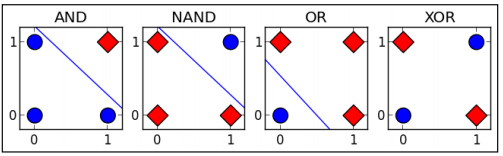
\includegraphics[width=0.4\textwidth]{figures/XOR_problem.png}
\caption{Residual Learning.}
\label{fig:1-1_residual_learning}
\end{figure}
 \uline{Linear classification models can't classify linear non-separable problems.} Perceptron is a linear classificatioin model, and XOR problem is a linear non-separable problem, so perceptron can't solve the XOR problem.

\subsection{Definition of perceptron}
Suppose the input space is $\mathcal{X} \subseteq \mathbb{R}^n$, and the output space is $\mathcal{Y} = \left\{+1, -1\right\}$. For an example $x \in \mathcal{X}$ where $x$ is an n-dimensional vector $(x_{1}, x_{2}, \cdot \cdot \cdot, x_{n})^\mathrm{T}$, $y \in \mathcal{Y}$ represents the category of $x$. Then, we get the perceptron model from the input space to output space: 
\begin{equation}
f(\vec{x}) = \mathrm{sign}(\vec{w}^\mathrm{T} \vec{x} + b),
\end{equation}
where $\vec{w}$ is weight and $b$ is bias. And $\mathrm{sign}$ is a sign function, $i. e.$
\begin{equation}
\mathrm{sign}(x)=
\left\{
	\begin{array}{ll}
		+1, \quad x \ge 0  \\
		-1, \quad x < 0
	\end{array}
\right.
\end{equation}

There exists \uline{a geometric interpretation} that a hyperpalne whose normal vector is $\vec{w}$ and intercept is $b$.

\subsection{Learning Algorithm}
Given a \uline{linear separable} dataset $T = {(x_{1}, y_{1}), (x_{2}, y_{2}), \cdot \cdot \cdot, (x_{N}, y_{N})}$, where $x_{i} \in \mathcal{X} \subseteq \mathbb{R}^n$, and $y_{i} \in \mathcal{Y} = {+1, -1}, i = 1, 2, \cdot \cdot \cdot, N$, we can construct a perspectron model to classify this dataset. 

(1) construct the loss function. we define the loss function as \uline{the total distance from misclassified points to hyperplane}. Toward this end, the distance from any point $x_{0}$ to hyperplane:
\begin{equation}
\frac{1}{||\vec{w}||} |\vec{w}^\mathrm{T}  \cdot \vec{x_{0}} + b|
\end{equation}
where ${||\vec{w}||}$ means the $L_{2}$ norm of $\vec{w}$.\\
\indent As for missclassified points, $\vec{w}^\mathrm{T}  \cdot \vec{x_{0}} + b > 0$ when $y_{i}=-1$, and $\vec{w}^\mathrm{T}  \cdot \vec{x_{0}} + b < 0$ when $y_{i}=+1$. So the total distance from all the misscalssified points to hyperplane is 
\begin{equation}\label{eq:perceptron_loss}
-\frac{1}{||w||}\sum_{\vec{x_{i}} \in M} y_{i} (\vec{w}^\mathrm{T}  \cdot \vec{x_{i}} + b),
\end{equation}
where $M$ is the set of misclassfied points.

\indent \uline{In Eq.~\ref{eq:perceptron_loss}, $\frac{1}{||w||}$ can be ignored. The reason is (a) $\frac{1}{||w||}$ doesn't affcet postive or negative judgment of $y_{i} (\vec{w}^\mathrm{T}  \cdot \vec{x_{i}} + b)$ and (b) $\frac{1}{||w||}$ doesn't affcet the final optimization result of Eq.~\ref{eq:perceptron_loss}. The final optimization result is there are no points with wrong classification, which leads to the loss of 0.} Toward this end, the loss function of preceptron is 
\begin{equation}\label{eq:perceptron_loss}
L(\vec{w}, b) = - \sum_{\vec{x_{i}} \in M} y_{i} (\vec{w}^\mathrm{T}  \cdot \vec{x_{i}} + b),
\end{equation}
and the optimization object is 
\begin{equation}\label{eq:perceptron_loss}
\min_{\vec{w}, b}L(\vec{w}, b) = \min_{\vec{w}, b}- \sum_{\vec{x_{i}} \in M} y_{i} (\vec{w}^\mathrm{T}  \cdot \vec{x_{i}} + b).
\end{equation}

(2) We adopt stochastic gradient descent algorithm to train the perceptron model. Suppose the set of misclassified points is fixed, thus the gradient of loss function $L(\vec{w}, b)$:
\begin{equation}
\begin{split}
	\nabla_{\vec{w}}L(\vec{w}, b) & = - \sum_{\vec{x_i} \in M} y_i \vec{x_i} \\
	\nabla_{b}L(\vec{w}, b)       & = - \sum_{\vec{x_i} \in M} y_i
\end{split}.
\end{equation}
So, the stratagies of $\vec{w}$ and $b$ based on one misclassified point are:
\begin{equation}\label{eq:perceptron_parameter_update}
\begin{split}
	\vec{w} & \gets \vec{w} + \eta y_i \vec{x} \\
	b & \gets b + \eta y_i
\end{split},
\end{equation}
where $\eta$ is the learning rate.

(3) The standard form of perceptron learing algorithm: \\
\indent	\indent input: \uline{linear seperable training set}: $T = \left\{ (x_1, y_1), (x_2, y_2), \cdots, (x_n ,y_n) \right\}$, where $\vec{x_i} \in \mathcal{X} \subseteq \mathbb{R}^n$ and $y_i \in \mathcal{Y} = \left\{-1, +1\right\}, i = 1, 2, \cdots, N$. In addition, the learning rate is denoted 
as $\eta (0 < \eta \le 1)$. \\
\indent \indent output: $\vec{w}, b$. And the perceptron model $f(\vec{x}) = \mathrm{sign}(\vec{w}^\mathrm{T} \vec{x} + b)$. \\
\indent \indent (a) choose initial values, $\vec{w_0}, b_0$, and usually $\vec{w_0} = 0, b_0 = 0$; \\
\indent \indent (b) choose one example $(\vec{x_i}, y_i)$ from the traning set; \\
\indent \indent (c) if $y_{i} (\vec{w}^\mathrm{T}  \cdot \vec{x_{i}} + b) \le 0$:
\begin{equation}
\begin{split}
\vec{w} & \gets \vec{w} + \eta y_i \vec{x} \\
	b & \gets b + \eta y_i
\end{split};
\end{equation} \\
\indent \indent (d)go to (b) until there are no misclassified points in training set.


(4) \note[inline]{The convergence of this algorithm about perceptron leraning can be proved, but it is not within the scope of this note at present.}

\subsection{Dual form of perceptron learning algorithm}
From Eq.~\ref{eq:perceptron_parameter_update}, $\vec{w}$ and $b$ are updated for many times. Suppose the number of updates about each example is $n_i (i = 1, 2, \dots N)$, and we define $\alpha_i = n_i \eta$. Then, the final learned $\vec{w}$ and $b$ can be expressed as
\begin{equation}
\begin{split}
	\vec{w} & = \sum_{i = 1}^{N} \alpha_i y_i \vec{x_i} \\
	b 		& = \sum_{i = 1}^{N} \alpha_i y_i
\end{split}.
\end{equation}

Then, we can obtain the dual form of perceptron learning algorithm.\\
\indent	\indent input: \uline{linear seperable training set}: $T = \left\{ (x_1, y_1), (x_2, y_2), \cdots, (x_n ,y_n) \right\}$, where $\vec{x_i} \in \mathcal{X} \subseteq \mathbb{R}^n$ and $y_i \in \mathcal{Y} = \left\{-1, +1\right\}, i = 1, 2, \cdots, N$. In addition, the learning rate is denoted 
as $\eta (0 < \eta \le 1)$. \\
\indent \indent output: $\vec{\alpha} = (\alpha_1, \alpha_2, \cdots, \alpha_N)^\mathrm{T}, b$. And the perceptron model $f(\vec{x}) = \mathrm{sign}(\sum_{j=1}^{N} \alpha_j y_j \vec{x_j}^\mathrm{T} \vec{x} + b )$. \\
\indent \indent (a) choose initial values, $\vec{\alpha}, b_0$, and usually $\vec{\alpha} = 0, b_0 = 0$; \\
\indent \indent (b) choose one example $(\vec{x_i}, y_i)$ from the traning set; \\
\indent \indent (c) if $y_{i} (\sum_{j=1}^{N} \alpha_j y_j \vec{x_j}^\mathrm{T} \vec{x} + b) \le 0$:
\begin{equation}
\begin{split}
\vec{\alpha_i} & \gets \alpha_i + \eta \\
	b & \gets b + \eta y_i
\end{split};
\end{equation} \\
\indent \indent (d)go to (b) until there are no misclassified points in training set.

\section{How to get the update rule of parameters of backpropagation in gradient descent algorithm?}
An intuitive and imprecise proof is as follows. Assuming that there is a differentiable loss function $\mathcal{L}$ on training set with respect to parameter $\vec{w} = (w_1, w_2, \cdots, w_n)$ of the training model. Then, the total increment of $\mathcal{L}$ is
\begin{equation}
\begin{split}
\Delta \mathcal{L} & = \frac{\partial \mathcal{L}}{\partial w_1} \Delta w_1 + \frac{\partial \mathcal{L}}{\partial w_2} \Delta w_2 + \cdots + \frac{\partial \mathcal{L}}{\partial w_n} \Delta w_n + o(\rho) \\
				   & \approx \frac{\partial \mathcal{L}}{\partial w_1} \Delta w_1 + \frac{\partial \mathcal{L}}{\partial w_2} \Delta w_2 + \cdots + \frac{\partial \mathcal{L}}{\partial w_n} \Delta w_n
\end{split}.
\end{equation}
Define $\nabla \mathcal{L}_{\vec{w}} = (\frac{\partial \mathcal{L}}{\partial w_1}, \frac{\partial \mathcal{L}}{\partial w_2}, \cdots, \frac{\partial \mathcal{L}}{\partial w_n})^\mathrm{T}$, which represents the vector of gradients. Therefore, 
\begin{equation}
\Delta \mathcal{L} \approx \nabla \mathcal{L}_{\vec{w}}^\mathrm{T} \cdot \Delta \vec{w}.
\end{equation}
Our goal is to reduce the loss function $\mathcal{L}$, which is equivalent to making the total increment $\Delta \mathcal{L}$ negative. Toward this end, construct 
\begin{equation}
\Delta \vec{w} = -\eta \nabla \mathcal{L}_{\vec{w}},
\end{equation}
which ensure that $\Delta \mathcal{L} \approx \nabla \mathcal{L}_{\vec{w}}^\mathrm{T} \cdot \Delta \vec{w} = - \eta ||\nabla \mathcal{L}_{\vec{w}}^\mathrm{T}||_2^2 \le 0$. So, the update rule of parameter $\vec{w}$ is 
\begin{equation}
\vec{w} \gets \vec{w} -\eta \nabla \mathcal{L}_{\vec{w}}.
\end{equation}
\uline{In other word, in gradient descent algorithm, the direction of parameter update is opposite to its gradient direction.}

\section{Generative model and discriminative model}
(1) Generative model: perceptron

\section{Support vector machine}
\improvement[inline]{Todo: SVM}

\improvement[inline]{Todo: Random forest}

\chapter{Deep Network}
\section{Why does residual learning work?}
\begin{figure}[h]
\centering
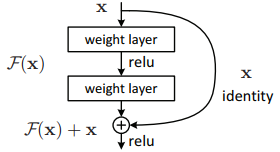
\includegraphics[width=0.2\textwidth]{figures/residual_learning_block.png}
\caption{Residual Learning.}
\label{fig:1-1_residual_learning}
\end{figure}

In the process of optimization in deep network, the input and output are usually close in the latter layers. In some latter layers, we define the input is $\rm{x}$ and the output is $\mathcal{H(\rm{x})}$. From above experience, we assume $\rm{x}$ and $\mathcal{H(\rm{x})}$ are close. Thus, the function of these layers is mapping from $\rm{x}$ to $\mathcal{H(\rm{x})}$. But usually this process is difficult becuase the relative gap between $\rm{x}$ and $\mathcal{H(\rm{x})}$ is small. Toward this end, we construct the residual as \uline{$\mathcal{F(\rm{x})} = \mathcal{H(\rm{x})} - \rm{x}$} to learning the gap. We can hypothesize that it is easier to optimize the residual mapping than to optimize the original mapping. To the extreme, if the mapping from input to output is indentity, it would be easier to push the residual to zero than to directly fit an identity mapping.

\uline{The real purpose of residual learning is that even if the network deepens, the performance of this network will not degenerate, thus ensuring the leaning of deeper network (even 1000 layers).}

\chapter{Contents specifically referenced}
$\bullet$ the chapter of (2)Perceptron in \cite{hangli2012};

{\small
\bibliographystyle{plain}
\bibliography{RefNote}
}

\end{document}
